\section{Biasedness of model}

From the previous 2 sections, we see that the posterior distributions for $B_a,B_b,B_c$ is actually not centered correctly.  To diagnosis this, I created a simplified model to isolate what was going wrong.  This is basically the part of the model that predicts $a$: 

\begin{eqnarray}
f^a(x) &=& \frac{1}{1+e^{-x}} \\
\mu_i^a &=& f^a(\mu_{pop}^a + B^ax_i) \\
a_i &\sim& Beta(\mu_i^a, \phi^a) \\
B &\sim& U(-\infty,\infty)
\end{eqnarray}

I generate 50 $x_i$'s centered symmetrically about 0.  I set $B_a=1$.  I obtain the corresponding $a_i$'s, with no noise, so that $a_i=\mu_i^a$.  I assume $\phi^a$ is fixed.  I do sampling to infer $P(B_a|a_i,x_i,\phi^a)$.  There is only 1 unobserved variable in this distribution - $B_a$.  The distribution of $P(B_a|a_i,x_i,\phi^a)$ changes as I vary $\phi^a$.  The distribution is centered correctly at 1.0 for small $\phi^a$.  The larger $\phi^a$ is, the more offset the distribution is.  See the following plot.

The reason for this biasedness is that if we fix $\phi^a$ to be large, the distribution for $a_i$ will be U-shaped.  I think posterior for $B_a$ is centered at 0 if $\phi^a$ is close to 1 because when the distribution of $a_i$ is U-shaped, it pays to be off in the predictions.  

\begin{figure}
\centering
\begin{subfigure}[$\phi^a=0.9$]{
  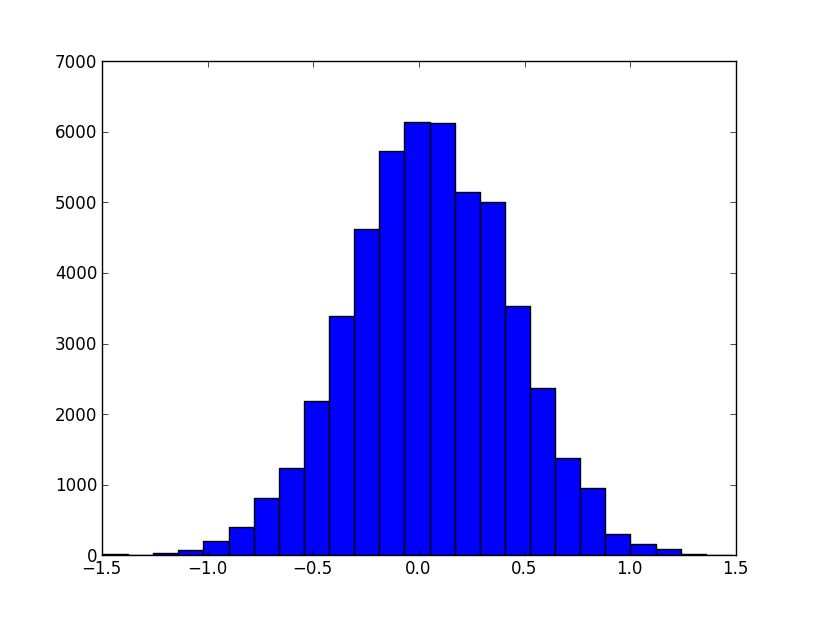
\includegraphics[width=.45\linewidth,height=0.3\textheight]{/Users/glareprotector/Documents/prostate/hist09.png}}
\end{subfigure}
\begin{subfigure}[$\phi^a=0.5$]{
  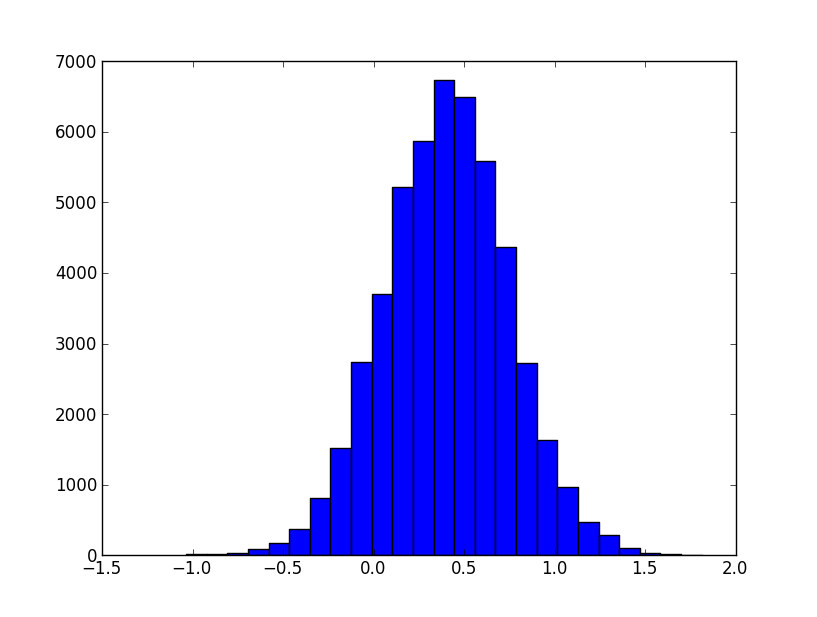
\includegraphics[width=.45\linewidth,height=0.3\textheight]{/Users/glareprotector/Documents/prostate/hist05.png}}
\end{subfigure}
\begin{subfigure}[$\phi^a=0.2$]{
  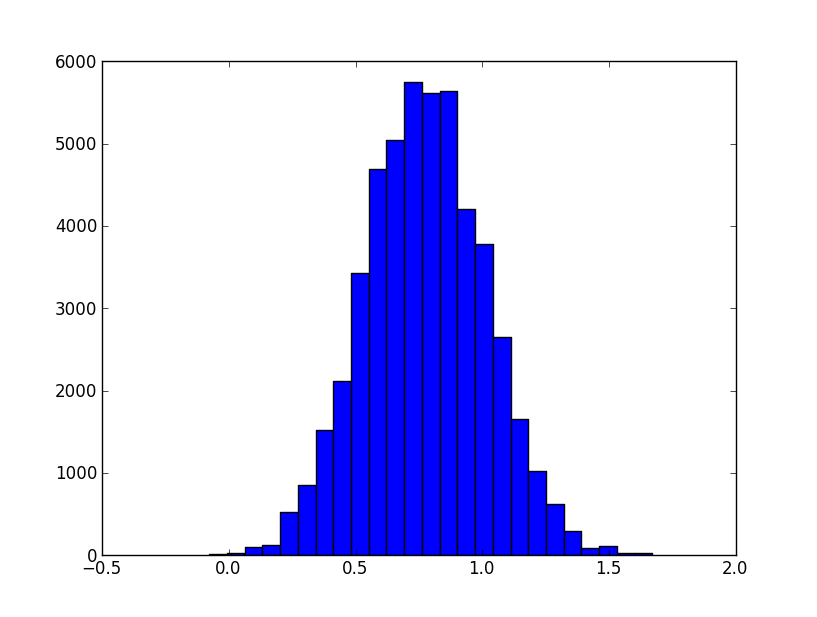
\includegraphics[width=.45\linewidth,height=0.3\textheight]{/Users/glareprotector/Documents/prostate/hist02.png}}
\end{subfigure}
\begin{subfigure}[$\phi^a=0.01$]{
  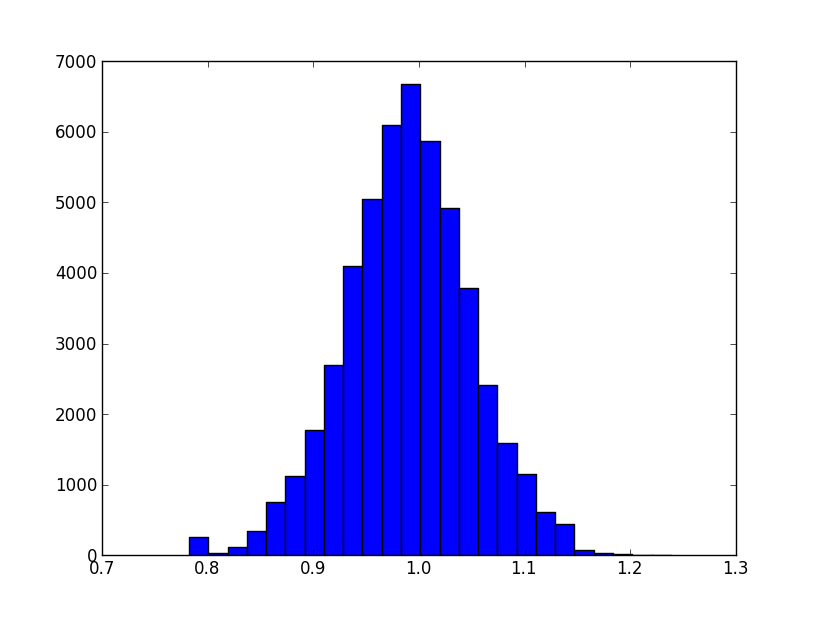
\includegraphics[width=.45\linewidth,height=0.3\textheight]{/Users/glareprotector/Documents/prostate/hist001.png}}
\end{subfigure}
\caption{histogram of posterior of $B_a$ when $\phi^a$ is fixed to various values during inference}
\end{figure}

The solution is to give zero probability to situations where the distribution of $P(a;\mu^a,\phi^a)$ is U-shaped.  This can be done by parameterizing the Beta distributions for $a$ and $b$ differently.  Before, $\phi^a$ represented the proportion of the maximum possible variance for a Beta distribution with the specified mean.  Now, we should let $\phi^a$ represented the proportion of the maximum possible variance for a Beta distribution with the specified mean, such that the distribution is still unimodal.  Hopefully this quantity can be calculated analytically.